\documentclass{article}
\usepackage[toc,page]{appendix}

\usepackage[preprint]{neurips_2023}
\usepackage[utf8]{inputenc} % allow utf-8 input
\usepackage[T1]{fontenc}    % use 8-bit T1 fonts
\usepackage{hyperref}       % hyperlinks
\usepackage{url}            % simple URL typesetting
\usepackage{booktabs}       % professional-quality tables
\usepackage{amsfonts}       % blackboard math symbols
\usepackage{nicefrac}       % compact symbols for 1/2, etc.
\usepackage{microtype}      % microtypography
\usepackage{xcolor}         % colors
\usepackage{hyperref}       % links

\usepackage{graphicx}       % include graphics
\usepackage{float}
\usepackage[T1]{fontenc}

\usepackage{caption}
\usepackage{subcaption}

\newcommand{\sais}{Scottish Avalanche Information Service}

\title{ML-based avalanche danger level forecasting. \\ Category: General Machine Learning}


\author{
  Witold Gawlikowicz (06932552) \\
  \texttt{witold@stanford.edu}
}


\begin{document}

\maketitle

\graphicspath{{assets/figures/}}


% \begin{abstract}
% \end{abstract}

% TODOs:
	% Go into details of what the snowpack data is

	% Milestone
	% The milestone will help you make sure you're on track, and should describe what you've accomplished so far, and very briefly say what else you plan to do. You should write it as if it's an “early draft" of what will turn into your final project. You can write it as if you're writing the first few pages of your final project report, so that you can re-use most of the milestone text in your final report. Please write the milestone (and final report) keeping in mind that the intended audience are the instructors and the TAs. Thus, for example, you should not spend two pages explaining what logistic regression is. Your milestone should include the full names of all your team members and state the full title of your project. Note: We will expect your final writeup to be on the same topic as your milestone.
	% Contributions
	% Please include a section that describes what each team member worked on and contributed to the project. This is to make sure team members are carrying a fair share of the work for projects. If you have any concerns working with one of your project teammates, please create a private Ed post.
	% Grading
	% The milestone is mostly intended to get feedback from TAs to make sure you’re making reasonable progress. As long as your milestone follows the instructions above and you seem to have tested any assumptions which might prevent your team from completing the project, you should do well on the milestone.
	% Format
	% Your milestone should be at most 3 pages, excluding references. Similar to the proposal, it should include
	% Motivation: What problem are you tackling, and what's the setting you're considering?
	% Method: What machine learning techniques have you tried and why?
	% Preliminary experiments: Describe the experiments that you've run, the outcomes, and any error analysis that you've done. You should have tried at least one baseline.
	% Next steps: Given your preliminary results, what are the next steps that you're considering?
	
	

\section*{Acknowledgements}

\section{Motivation}

	Every year around a 100 people loose their lives to avalanches \href{https://www.avalanches.org/fatalities/}{in Europe alone} despite the fact that avalanche danger level forecasts are widely available there. There are many mountainous regions around the world for which no such forecasts are published.
	Automating the process of avalanche forecast generation could have real impact on lives of many people around the world. \\
	This is of course an extremely ambitious goal, well beyond the scope of even most exhaustive coursework project. However, as I'm a keen alpinist and this topic if very close to my heart, I'd like to explore how much I can achieve towards this goal over the next 7 weeks and open-source it for the benefit of other researchers, as well as potentially continue working on it beyond CS229.

	The main part of the avalanche danger level forecast for a given region is the overall avalanche danger level. It's expressed on a 5 point scale ranging from 1 (lowest) to 5 (highest).	\href{https://www.shastaavalanche.org/page/how-read-advisory}{Forecasts} for many regions often also contain: \href{https://avalanche.state.co.us/forecasts/tutorial/avalanche-problems}{the avalanche problems} (main characteristics of the snowpack which contribute to its instability and hence potential avalanche) and the aspect-elevation rose which shows more fine-grained avalanche danger levels broken down by slope's aspect and elevation. \\
	My primary goal is to use the overall avalanche danger level forecast for the region as the dependent variable, however time- and data-permitting I'd also like to explore the possibility generating those more detailed elements of an avalanche forecast.	
	
	While I'm very enthusiastic about the topic, my biggest reservations were to do with the availability of data. However, my initial exploration has yielded some promising datasets. \href{https://www.sais.gov.uk/forecast-archive/}{Scottish Avalanche Information Service} provides historical forecasts for 5 regions since 1993 which we estimate to contain around 15,000 forecasts (typically the avalanche centres don't publish forecasts throughout the entire year). I have also been in touch with the \href{https://avalanche.org/national-avalanche-center/}{US Forest Service National Avalanche Center} and was told that it should be possible to obtain a dataset containing avalanche forecasts from the last 10 years from all of the avalanche centres in the US. \\
	For the independent variables I'd like to use the weather variables typically associated with formation of avalanche problems (precipitation, temperature and wind activity across the season). I'd like to use the data source that provides historical and current results across the globe so that the methodology could be used to generate forecasts for regions which currently don't benefit from any official forecasts. I haven't yet decided which source to use, but from my initial search it seems like it should be possible to find a suitable one.
	
	I'd like to start with a simple softmax regression as a baseline and then compare its performance with more complex models. I'm also considering replicating some of the results presented in \citation{nhess-22-2031-2022} using the datasets obtained for this project. I'll evaluate the model by calculating the difference between the predicted and actual avalanche danger level on a pre-assigned validation subset of the data. 
	

\section{Data}

	This section briefly describes the datasets collected to date.

\subsection{\sais}

	The \href{https://www.sais.gov.uk/forecast-archive/}{Scottish Avalanche Information Service} (SAIS) provides historical avalanche forecasts for 6 regions in Scotland. The forecasts are typically published from December to April. SAIS allows bulk download of snowprofile data containing both observed (nowcast) and forecasted avalanche hazard level as well as snowprofile data collected during compilation of observed hazard levels. The size of the dataset prior to any cleansing is \input{assets/snippets/sais_size_initial.txt}observations.
	\newline
	The dataset contains two variables either of which could be used as our dependent variable: observed and forecasted avalanche hazard level.
	The forecasted value is composed by avalanche professionals working in a given area based on the current state of the snowpack and the weather forecast for the next day.
	The observed value (nowcast) is decided on the day after a field trip in the area for which the avalanche hazard level is being assessed and taking one or more measurements of the snowpack (by digging snow profiles).
	\newline
	While both values are composed used a standardised methodology, there's inherent subjectivity in both of them, but especially so in the nowcast as it relies a lot on travel throughout the area and multifaceted, in-person assessment of the snow conditions. For that reason we will use the forecasted value as our dependent value as it should be more standardised, have a clearer relationship with the weather inputs and thus be more feasible for the model to discover the underlying relationship between the variables.

\subsubsection{Initial transformation}
	We have dropped missing values of both potential independent variables and used various strategies for filling missing data (details can be found if Table \ref{tbl:sais_replacements_log}). Brining the number of observations from \input{assets/snippets/sais_size_initial.txt} to \input{assets/snippets/sais_size_final.txt}
\subsubsection{Splits}
	As seen in Table \ref{tbl:sais_area_breakdown} the "Torridon" region only has relevant observations present present from the 2013/2014 winter season (as opposed to the other ones for which relevant observations are present from 2007/2008 season onwards). 
	Because of that the region has fewest observations and might have different characterstics due to changes in methodology and climate over time. For that reason we have decided to use it as a test set to see how well the models generalize into other regions (and to some extent different time frames).
	While it would be nice to be able to test how well models generalize to other time frames for the data from the same regions as they were trained on we have decided not to withold any data for that purpose not to reduce the size of the remaining datasetset any further. This data will start appearing for the 2024/2025 winter season soon, so we will extend the dataset with it when available.
	\newline
	We have used 20\% of the remaining data as the development set stratifying on both the areas and avalanche hazard levels. The resulting split is presented in the table below:

	\begin{table}[H]
\centering
\caption{\detokenize{"mapped_hazard_forecast"} per dataset split}
\label{tbl:sais_hazard_breakdown_per_split}
\begin{tabular}{rrrr}
\toprule
\detokenize{mapped hazard forecast} & Train & Dev & Test \\
\midrule
1 & 2073 & 518 & 545 \\
2 & 2070 & 517 & 405 \\
3 & 2476 & 620 & 131 \\
4 & 380 & 95 & 1 \\
\bottomrule
\end{tabular}
\end{table}


	Breakdown of hazard levels per each area in Training and Development sets can be found in Tables \ref{tbl:sais_mapped_hazard_breakdown_per_area_train} and \ref{tbl:sais_mapped_hazard_breakdown_per_area_dev}

\subsection{US Forest Service National Avalanche Center}

\section{Metrics}

	To begin with with will consider accuracy, precision, recall and F-1 score as the primary metrics for evaluating the model. Accuracy works the same as in the binary classification case, but the other metrics will need to be calculated per class (considering a given class vs all others). We will also plot the confusion matrices for different models and include them in the appendix.
	In the later part of the project we might also consider other metrics, such as macro- and micro-averaged of the above per-class metrics.
	\newline
	We might also consider other metrics that would allow us to capture if a given model tends to over- or under-report the hazard level as, if having to choose between the two, a general 
	preference would be towards over-reporting for a system used to predict hazards (so it's users are rather overly cautious than overlyoptimistic about the conditions). 


\subsection{Baseline fits}

	To get a better feel for how the different metrics are behaving on this dataset we will compute two baselines: 
	\begin{enumerate}
		\item A constant model that always predicts the most common class in the test set.
		\item Evaluate different metrics on the mapped values of observed vs forecasted avalanche danger levels present in the test set.
	\end{enumerate}
	The idea is that the first baseline will provide a lower bound on the performance of any model we might want to seriously consider and the second one will likely be the upper bound as it's compiled by the same experts who made the forecast, but with the additional benefit of being able to directly observe the actual changes in the snowpack.

	Metrics for those baselines and all the models considered will be included in Section \ref{sec:evaluation}.

\section{Model Fitting}

	In this section, we describe the process of fitting machine learning models to the collected data. We start with a simple softmax regression model as a baseline and then explore more complex models.

\subsection{Softmax Regression}

	Softmax regression, also known as multinomial logistic regression, is a generalization of logistic regression to multiple classes. It is a simple and interpretable model that serves as a good starting point.

\section{Evaluation}\label{sec:evaluation}
	The evaluation metrics for each model computed on the test are presented below. Please refer to the appendix for equivalent tables for the development sets.
	\begin{table}[H]
\caption{Evaluation metrics computed on the test set}
\label{tbl:sais_eval_test}
\begin{tabular}{lllll}
\toprule
 & constant & observed & softmax regression (snow profiles) & softmax regression (snow profiles tabularised) \\
\midrule
MSE & 2.4 & 0.2 & 0.3 & 1.9 \\
average error & -1.4 & 0.1 & 0.0 & -0.7 \\
highest error & -2 & 2 & 2 & -3 \\
accuracy & 0.1 & 0.8 & 0.7 & 0.3 \\
precision (multiclass) & [0.0, 0.0, 0.12, 0.0] & [0.82, 0.78, 0.89, 0.0] & [0.79, 0.65, 0.43, 0.0] & [0.55, 0.39, 0.13, 0.01] \\
precision (micro) & 0.1 & 0.8 & 0.7 & 0.3 \\
precision (macro) & 0.0 & 0.6 & 0.5 & 0.3 \\
recall (multiclass) & [0.0, 0.0, 1.0, 0.0] & [0.93, 0.71, 0.63, 0.0] & [0.88, 0.46, 0.63, 0.0] & [0.3, 0.25, 0.39, 1.0] \\
recall (micro) & 0.1 & 0.8 & 0.7 & 0.3 \\
recall (macro) & 0.2 & 0.6 & 0.5 & 0.5 \\
$F_1$ (multiclass) & [0.0, 0.0, 0.22, 0.0] & [0.87, 0.74, 0.74, 0.0] & [0.84, 0.54, 0.51, 0.0] & [0.39, 0.31, 0.2, 0.01] \\
$F_1$ (micro) & 0.1 & 0.8 & 0.7 & 0.3 \\
$F_1$ (macro) & 0.1 & 0.6 & 0.5 & 0.2 \\
\bottomrule
\end{tabular}
\end{table}


\section{Next steps}
	Please note that some of these are nice to haves, I very likely will not manage to go though all of them in the time available (though I am keen to continue working on this problem beyond this term):
	\begin{itemize}
		\item Expolore performance of more complex models. 
		\item Look into APIs for historical weather data.
		\item If historical data is available revisit SAIS dataset and train it on: mixture of existing snowprofiles and weather data, weather data only, [simulated snow profiles](https://snowpack.slf.ch).
		\item If the above shows promise re-run it on US Forrest Service dataset.
		\item See if it's possible to use data relating to observations of snowpack at different points to add more granularity to the model (still predict overall hazard level for a forecast area, but see if it can be locally raised or lowered depening on aspects, elevations, angles and altitudes).
		\item Visualise predictions on a map.
	\end{itemize}

\newpage
\begin{appendices}
	\section{Dataset details}
	This section contains further details of the datasets used for the project.

	\subsection{\sais}
	
	\begin{table}[H]
\caption{Summary of the SAIS dataset prior to any modifications}
\label{tbl:sais_summary_initial}
\begin{tabular}{rrllll}
\toprule
non-null & unique & dtype & mean & min & max \\
\midrule
17453 & 12045 & datetime64[ns] & 2011-03-06 & 1993-12-20 & 2024-04-13 \\
17453 & 6 & object & NaN & NaN & NaN \\
11402 & 791 & object & NaN & NaN & NaN \\
11291 & 3557 & object & NaN & NaN & NaN \\
17434 & 683 & object & NaN & NaN & NaN \\
17095 & 337 & float64 & 97.1 & -1.0 & 163770.0 \\
17384 & 56 & float64 & 17.8 & -1.0 & 1020.0 \\
11409 & 3497 & object & NaN & NaN & NaN \\
17389 & 520 & object & NaN & NaN & NaN \\
17221 & 366 & float64 & 199.0 & -9999.0 & 905.0 \\
17376 & 107 & float64 & 14.2 & -9999.0 & 360.0 \\
17402 & 38 & float64 & 73.3 & -9999.0 & 199.0 \\
10756 & 9 & object & NaN & NaN & NaN \\
17452 & 6 & object & NaN & NaN & NaN \\
17194 & 279 & float64 & 65.3 & -1.0 & 3000.0 \\
17380 & 87 & float64 & 1.0 & -9999.0 & 310.0 \\
14028 & 28 & float64 & 0.4 & -1.0 & 55.0 \\
17453 & 3 & int64 & -11.3 & -9999.0 & 1.0 \\
16253 & 222 & float64 & -0.8 & -13.4 & 15.0 \\
15638 & 357 & float64 & 123.4 & -2.0 & 2213.0 \\
16039 & 153 & float64 & 17.7 & -8.0 & 360.0 \\
11310 & 6 & object & NaN & NaN & NaN \\
11792 & 6 & object & NaN & NaN & NaN \\
17090 & 214 & object & NaN & NaN & NaN \\
16811 & 120 & float64 & 1.2 & 0.0 & 130.0 \\
16886 & 8 & float64 & 1.3 & 0.0 & 5.0 \\
16714 & 368 & float64 & 149.8 & -9999.0 & 676.0 \\
16234 & 58 & float64 & -3.8 & -9999.0 & 368.0 \\
16480 & 22 & float64 & -1.4 & -9999.0 & 208.0 \\
15988 & 11 & float64 & -6.8 & -9999.0 & 20.0 \\
16401 & 11 & float64 & -3.9 & -9999.0 & 10.0 \\
14457 & 20 & float64 & -3071.0 & -9999.0 & 8800.0 \\
16574 & 284 & float64 & -6.1 & -9999.0 & 125.0 \\
13736 & 5917 & object & NaN & NaN & NaN \\
\bottomrule
\end{tabular}
\end{table}

	
	\begin{figure}[h]
		\centering
		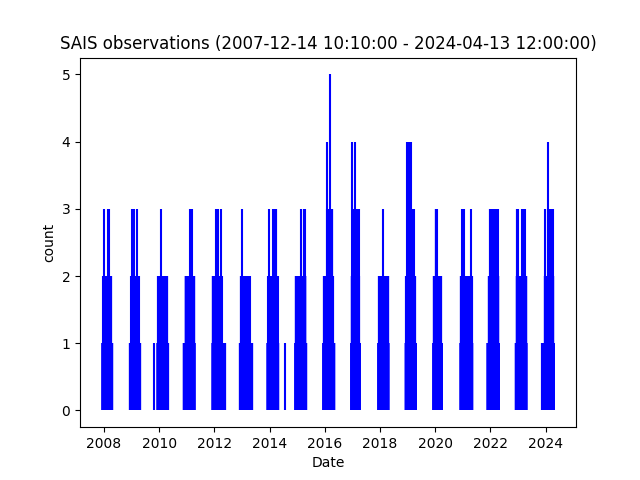
\includegraphics[width=0.7\textwidth]{sais_observation_histogram.png}
		\caption{Histogram of avalanche danger levels in the SAIS dataset.}
		\label{fig:sais_observation_histogram}
	\end{figure}

	\begin{table}[h]
\caption{Count of hazard levels and date ranges per area after dropping missing hazard values.}
\label{tbl:sais_area_breakdown}
\begin{tabular}{lrll}
\toprule
 & total & min date & max date \\
Area &  &  &  \\
\midrule
Creag Meagaidh & 1973 & 2007-12-21 & 2024-04-13 \\
Glencoe & 1991 & 2007-12-21 & 2024-04-13 \\
Lochaber & 2092 & 2007-12-14 & 2024-04-13 \\
Northern Cairngorms & 2125 & 2007-12-14 & 2024-04-13 \\
Southern Cairngorms & 1994 & 2007-12-21 & 2024-04-13 \\
Torridon & 1108 & 2013-12-24 & 2024-04-13 \\
\bottomrule
\end{tabular}
\end{table}

	\begin{table}[h]
\caption{"Forecast aval. hazard" breakdown per area area after dropping missing hazard values.}
\label{tbl:sais_hazard_breakdown_per_area}
\begin{tabular}{lrrrrr}
\toprule
 & Considerable + & Considerable - & High & Low & Moderate \\
Area &  &  &  &  &  \\
\midrule
Creag Meagaidh & 299 & 478 & 125 & 462 & 609 \\
Glencoe & 231 & 504 & 139 & 559 & 558 \\
Lochaber & 225 & 615 & 147 & 544 & 561 \\
Northern Cairngorms & 295 & 534 & 111 & 546 & 639 \\
Southern Cairngorms & 153 & 493 & 96 & 662 & 590 \\
Torridon & 13 & 126 & 1 & 549 & 419 \\
\bottomrule
\end{tabular}
\end{table}

	\begin{table}[h]
\caption{\detokenize{"mapped_hazard_forecast"} breakdown per area}
\label{tbl:sais_mapped_hazard_breakdown_per_area}
\begin{tabular}{lrrrr}
\toprule
 & 1 & 2 & 3 & 4 \\
Area &  &  &  &  \\
\midrule
Creag Meagaidh & 462 & 609 & 777 & 125 \\
Glencoe & 559 & 558 & 735 & 139 \\
Lochaber & 544 & 561 & 840 & 147 \\
Northern Cairngorms & 546 & 639 & 829 & 111 \\
Southern Cairngorms & 662 & 590 & 646 & 96 \\
Torridon & 549 & 419 & 139 & 1 \\
\bottomrule
\end{tabular}
\end{table}

	\begin{table}[H]
\caption{Summary of data cleansing actions on SAIS dataset}
\label{tbl:sais_replacements_log}
\begin{tabular}{ll}
\toprule
column name & action \\
\midrule
Forecast aval. hazard & 5661 missing values dropped \\
Observed aval. hazard & 509 missing values dropped \\
Air Temp & Change datatype to numeric \\
Drift & Change datatype to numeric \\
Summit Wind Dir & Set to 0 if "Summit Wind Speed" = 0 \\
Wind Dir & Set to 0 if "Wind Dir" = 0 \\
Summit Air Temp & Cross fill missing values with "Air Temp" \\
Summit Wind Dir & Cross fill missing values with "Wind Dir" \\
Summit Wind Speed & Cross fill missing values with "Wind Speed" \\
Precip Code & 605 NAs filled with "0 - None" \\
Foot Pen & 33 NAs filled with "0" \\
Ski Pen & 3356 NAs filled with "0" \\
Crystals & 1414 NAs filled with "0" \\
Wind Speed & 18 NAs filled with "0" \\
Summit Wind Speed & 18 NAs filled with "0" \\
Total Snow Depth & 221 NAs filled with "0" \\
Max Temp Grad & 557 NAs filled with "0" \\
Max Hardness Grad & 482 NAs filled with "0" \\
Snow Index & 1180 NAs filled with "0" \\
Wetness & 997 NAs filled with "0" \\
Precip Code & Split into "\detokenize{precip_code_numeric}" and "\detokenize{precip_code_desc}" \\
All columns & Drop 1049 with missing values \\
Wind Dir & Drop 15 negative values \\
Wind Speed & Drop 2 negative values \\
Cloud & Drop 1 negative values \\
Total Snow Depth & Drop 36 negative values \\
Foot Pen & Drop 2 negative values \\
Ski Pen & Drop 4 negative values \\
Summit Wind Dir & Drop 184 negative values \\
Summit Wind Speed & Drop 5 negative values \\
Snow Index & Drop 64 negative values \\
Insolation & Drop 2 negative values \\
Crystals & Drop 77 negative values \\
No Settle & Drop 4 negative values \\
Wetness & Drop 7 negative values \\
\bottomrule
\end{tabular}
\end{table}

	\begin{table}[h]
\caption{Training set: \detokenize{"mapped_hazard_forecast"} breakdown per area}
\label{tbl:sais_mapped_hazard_breakdown_per_area_train}
\begin{tabular}{lrrrr}
\toprule
 & 1 & 2 & 3 & 4 \\
Area &  &  &  &  \\
\midrule
Creag Meagaidh & 319 & 355 & 376 & 42 \\
Glencoe & 437 & 417 & 543 & 103 \\
Lochaber & 433 & 440 & 647 & 114 \\
Northern Cairngorms & 426 & 478 & 610 & 79 \\
Southern Cairngorms & 458 & 380 & 300 & 42 \\
\bottomrule
\end{tabular}
\end{table}

	\begin{table}[H]
\caption{Development set: \detokenize{"mapped_hazard_forecast"} breakdown per area}
\label{tbl:sais_mapped_hazard_breakdown_per_area_dev}
\begin{tabular}{lrrrr}
\toprule
 & 1 & 2 & 3 & 4 \\
Area &  &  &  &  \\
\midrule
Creag Meagaidh & 46 & 46 & 40 & 6 \\
Glencoe & 65 & 61 & 63 & 15 \\
Lochaber & 54 & 51 & 80 & 18 \\
Northern Cairngorms & 50 & 56 & 90 & 6 \\
Southern Cairngorms & 48 & 41 & 35 & 2 \\
Torridon & 50 & 44 & 15 & 1 \\
\bottomrule
\end{tabular}
\end{table}


	\section{Evaluation}
	\begin{figure}[h]
		\centering
		\begin{subfigure}[t]{0.49\textwidth}
			\centering
			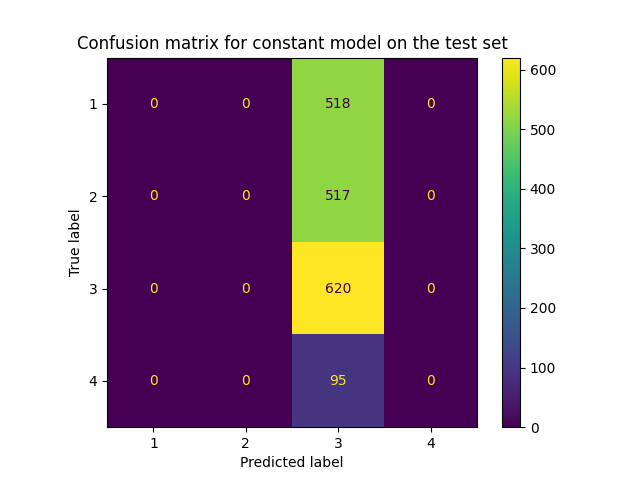
\includegraphics[width=\textwidth]{sais_confusion_matrix_constant_test.png}
			\caption{Test set}
		\end{subfigure}
		\hfil
		\begin{subfigure}[t]{0.49\textwidth}
			\centering
			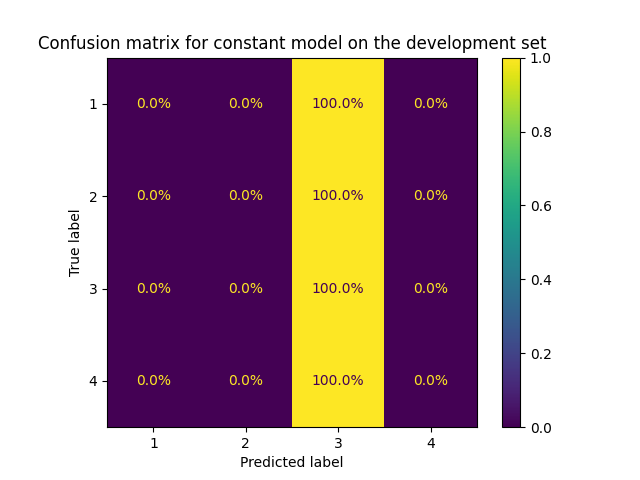
\includegraphics[width=\textwidth]{sais_confusion_matrix_constant_development.png}
			\caption{Development set}
		\end{subfigure}
		\caption{Constant model}
	\end{figure}

	\begin{figure}[h]
		\centering
		\begin{subfigure}[t]{0.49\textwidth}
			\centering
			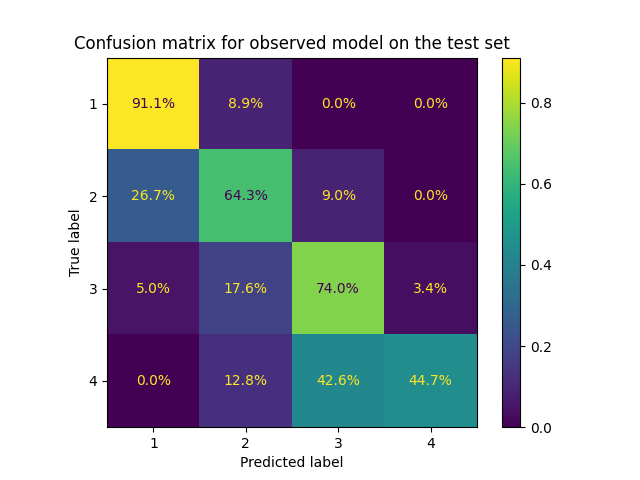
\includegraphics[width=\textwidth]{sais_confusion_matrix_observed_test.png}
			\caption{Test set}
		\end{subfigure}
		\hfil
		\begin{subfigure}[t]{0.49\textwidth}
			\centering
			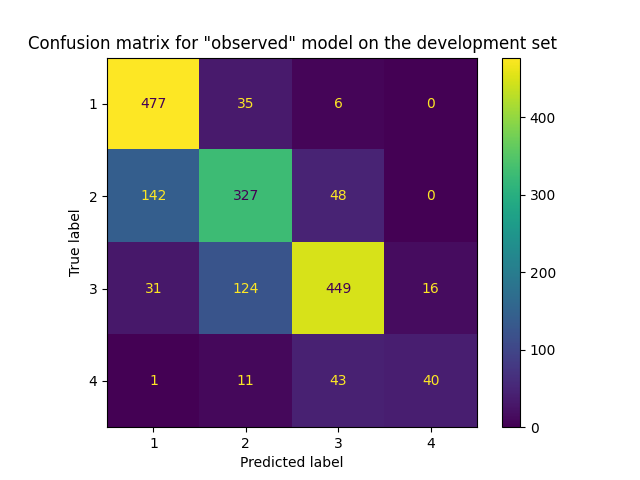
\includegraphics[width=\textwidth]{sais_confusion_matrix_observed_development.png}
			\caption{Development set}
		\end{subfigure}
		\caption{"Observed" model}
	\end{figure}

\end{appendices}
	

% \bibliographystyle{plainnat}  
% \bibliography{references}   
\nocite{*}
\bibdata{references}
\bibstyle{plainnat}  
\end{document}

	% Leftovers:
	%	As the number of people participating in outdoor recreation is \href{https://americancanoe.org/wp-content/uploads/2023/06/2023_Outdoor_Participation_Trends_Report.pdf}{steadily growing in the US}, and likely most of the other countries with access to mountains too, a
	%	On a \href{https://avalanche.org/avalanche-encyclopedia/human/resources/north-american-public-avalanche-danger-scale/}{North American scale} the levels are: 1 - "low", 2 - "moderate", 3 - "considerable", 4 - "high", 5 - "extreme". 
	%	The \href{https://www.avalanches.org/standards/avalanche-danger-scale/}{European scale} is similar with level 5 being described as "very high". Due to the ongoing efforts of the global avalanche forecasting scientific community the forecasting terminology have been getting more standardised across the world. However, it has to be noted that regional difference may still be present. 
	%	aspect ("N", "NE", "E", "SE", "S", "SW", "W", "NW") and elevation (either absolute elevations applicable to a given region or relative elevations driven by tree cover: "below treeline", "near treeline", "above treeline").
	